\chapter{Needfinding}

\begin{redbar}
Il termine \textbf{needfinding} si riferisce all'attività di identificare le necessità potenziali degli utenti e le lacune nei sistemi attuali, per trovare opportunità di miglioramento. E' importante non solo riconoscere i problemi esistenti, ma anche identificare come questi possono trasformarsi in opportunità per creare soluzioni migliori.
\end{redbar}

Nel contesto del design centrato sull'utente (Human-Centered Design), il needfinding è uno dei primi passi essenziali. Si tratta di un processo esplorativo, dove i progettisti cercano di scoprire i bisogni latenti degli utenti, osservando attentamente i loro comportamenti e le interazioni con i sistemi attuali. Non ci si limita a chiedere agli utenti cosa desiderano, ma si esplora il contesto in cui operano e come utilizzano i prodotti esistenti.

\begin{figure}[ht]
    \centering
    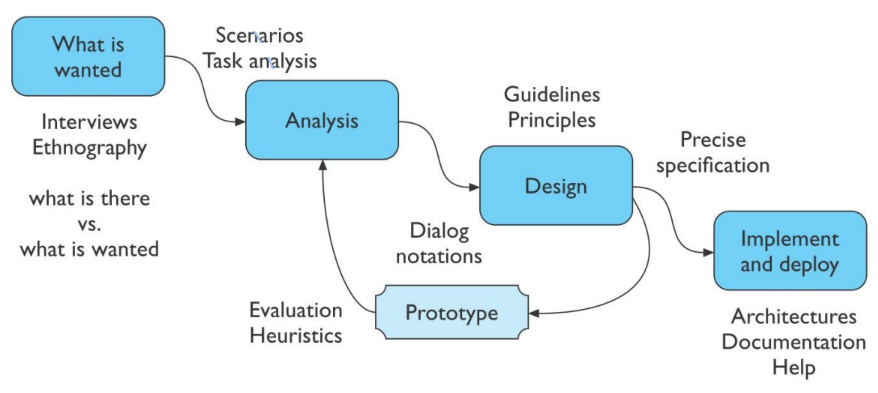
\includegraphics[width=0.7\textwidth]{images/human-centered-design-process.png}
    \caption{Human-Centered Design Process}
    \label{fig:human-centered-design-process}
\end{figure}

Il needfinding si concentra nel riconoscere i "vuoti" o gap all'interno di un sistema. Un esempio pratico di questo concetto è rappresentato dalla ricerca su come le persone utilizzano un'applicazione di benessere digitale. Attraverso l'osservazione, possiamo identificare problemi che magari gli utenti non esprimono apertamente, come difficoltà nell'uso o comportamenti di adattamento (\textit{workaround}). Questo processo permette ai progettisti di rispondere a domande fondamentali come: \textit{Chi sono gli utenti? Come stanno utilizzando il sistema ora? In quale contesto lo usano?}

Per condurre un’efficace attività di needfinding, è cruciale identificare correttamente i veri utenti. Un errore comune è presumere che i progettisti stessi o i clienti del progetto siano utenti rappresentativi, ma in realtà le loro competenze e conoscenze sono molto diverse. Bisogna invece parlare con le persone che effettivamente useranno il sistema.

\section{Metodi di needfinding}
Uno dei metodi più utilizzati per raccogliere informazioni è parlare direttamente con gli utenti. Si possono usare tecniche come interviste, questionari o coinvolgimento diretto nel processo di design. E' importante comprendere il comportamento reale degli utenti, ascoltando attentamente i loro problemi e cercando di cogliere le soluzioni che adottano per superare le difficoltà (workaround).

\subsection{Osservazione}
L’\textit{osservazione} è uno strumento fondamentale. Si tratta di osservare il comportamento degli utenti in modo naturale, senza interferenze. Un classico esempio è lo studio etnografico, che consiste nell'immergersi nel contesto dell'utente per capire meglio come funziona l'ambiente in cui opera. L'obiettivo è raccogliere dati che influenzeranno il redesign dell'interfaccia, imparando il "linguaggio" dell'utente e del suo ambiente.

Un altro punto importante che emerge riguarda la differenza tra processo e pratica. Il processo rappresenta il modo in cui le cose dovrebbero essere fatte ufficialmente, secondo la formazione, mentre la pratica riflette i trucchi appresi sul campo. Ad esempio, un impiegato potrebbe avere un metodo ufficiale per completare una determinata operazione, ma nel corso del tempo ha sviluppato delle scorciatoie o soluzioni personali che lo aiutano a lavorare più velocemente.

Esistono due principali tipi di osservazione: quella controllata in un ambiente di laboratorio e quella naturalistica sul campo. La prima è più facile da riprodurre e analizzare, poiché i dati sono spesso quantitativi e replicabili. Tuttavia, la seconda offre un contesto più realistico, permettendo agli utenti di affrontare le reali difficoltà che incontrano nella vita quotidiana. Ad esempio, l'osservazione di una persona che utilizza uno smartphone in condizioni di pioggia potrebbe rivelare sfide che non emergerebbero in laboratorio. La raccolta dei dati può essere di due tipi: soggettiva (basata su impressioni, valutazioni e racconti degli utenti) o oggettiva (come i dati registrati automaticamente da un sistema). Entrambi i tipi sono utili per costruire un quadro completo delle necessità degli utenti.

Tra i rischi dell'osservazione vi è il cosiddetto effetto \textit{hawthorne}, dove la semplice presenza dell'osservatore modifica il comportamento dell'utente. Per questo, è fondamentale adottare tecniche che riducano l'impatto dell'osservatore, come il \textit{blending in} (letteralmente, "confondersi con l’ambiente").

Come ha ben sintetizzato Uri Levine, fondatore di Waze: \textit{"Innamorati del problema, non della soluzione"}. Questa frase evidenzia quanto sia essenziale comprendere il vero problema, piuttosto che innamorarsi di una soluzione predefinita. L’osservazione, infatti, consente di definire con maggiore precisione il problema, e permette di scoprirlo in modo autentico e senza preconcetti.
L'osservazione, infatti, deve essere condotta con una mente aperta, senza cercare conferme per idee o soluzioni a priori. Bisogna essere pronti a scoprire dettagli imprevisti e lasciarsi sorprendere. Per questo motivo, l’osservatore deve prestare attenzione non solo a cosa fanno gli utenti, ma anche a quali sono i loro obiettivi, che strumenti utilizzano, il contesto in cui operano e le attività più ampie di cui fanno parte.
Quando si osservano gli utenti, è fondamentale non limitarsi a ciò che stanno facendo in quel preciso momento. Bisogna cercare di capire il loro obiettivo finale e come esso si collega all’attività specifica. E' altrettanto importante considerare il contesto in cui si trovano, inclusi fattori come il momento della giornata, l’ambiente fisico e le differenze tra gli utenti stessi. Dettagli come questi possono rivelare problematiche nascoste o opportunità di miglioramento.

Un metodo classico di osservazione è quello di passare del tempo vicino all’utente senza disturbarlo, lasciandolo agire naturalmente. Questo può essere fatto in luoghi pubblici come strade, locali o mezzi di trasporto, oppure attraverso l’analisi di video registrati, che consente uno studio più approfondito del comportamento senza interferenze dirette.
Un altro approccio importante è quello di “mettersi nei panni” dell'utente, partecipando attivamente alle loro attività. In questo modo, si possono scoprire dettagli che sfuggirebbero a un’osservazione passiva. Bisogna prestare particolare attenzione a eventuali trucchi, scorciatoie o errori commessi dagli utenti. Lavorare insieme a loro permette di ottenere una comprensione profonda dei loro reali bisogni.
Ascoltare gli utenti è tanto importante quanto osservarli. Spesso, ciò che gli utenti esprimono verbalmente non coincide esattamente con le loro azioni. Gli osservatori devono evitare di influenzare le risposte degli utenti con domande dirette o intrusive e concentrarsi invece su emozioni, paure e frustrazioni. Questo approccio consente di ottenere una visione più autentica e genuina dei bisogni degli utenti.

E' fondamentale non confondere i need (bisogni) con le soluzioni. I bisogni sono la chiave per aprire nuove opportunità, mentre le soluzioni possono limitare l’innovazione. Partire con una soluzione già in mente rischia di impedire l’immaginazione di qualcosa di completamente nuovo o rivoluzionario. La pazienza è cruciale, perché anche se le osservazioni possono sembrare inizialmente banali, è proprio nei piccoli dettagli che si possono nascondere intuizioni preziose.

\subsection{Diari}
Il metodo dei diari è utile quando non è possibile osservare direttamente gli utenti per lunghi periodi di tempo. In questo caso, si richiede agli utenti di tenere traccia delle loro attività quotidiane, annotando le azioni rilevanti. I diari possono essere cartacei o digitali, e gli utenti registrano le loro azioni quando eseguono specifiche operazioni o a intervalli di tempo prestabiliti.

L'uso dei diari consente di raccogliere dati su un lungo periodo di osservazione, fornendo informazioni dettagliate che potrebbero sfuggire in una semplice sessione di osservazione. Tuttavia, mantenere la motivazione degli utenti è essenziale: potrebbe essere utile offrire incentivi per assicurarsi che completino correttamente il diario.

\subsection{Interviste}
Le interviste sono un altro metodo importante per raccogliere dati dagli utenti. Si può scegliere tra interviste strutturate (con domande predeterminate) e non strutturate (che lasciano maggiore libertà). Le interviste possono essere condotte faccia a faccia o in gruppo (focus group). Rispetto ai sondaggi, le interviste permettono di ottenere conoscenze più profonde e dettagliate, ma richiedono molto tempo.

Un rischio delle interviste è che gli utenti potrebbero non sapere cosa vogliono realmente o potrebbero cercare di rispondere ciò che pensano l'intervistatore voglia sentire. Inoltre, per prodotti o tecnologie completamente nuove, gli utenti potrebbero non avere la creatività necessaria per immaginare potenziali applicazioni. Infatti, gli utenti spesso non riescano a esprimere esplicitamente i loro bisogni. Ad esempio, prima dell’invenzione dell'iPhone, nessuno avrebbe chiesto un telefono touch-screen con app, perché nessuno poteva immaginare quel prodotto. Questo evidenzia l'importanza di andare oltre le semplici richieste degli utenti e investigare i loro bisogni più profondi.

Nella scelta dei partecipanti alle interviste, è essenziale includere rappresentanti del target di utenti. In alcuni casi, può essere utile coinvolgere utenti attuali di sistemi simili, oppure anche i non utenti, se si sta progettando un prodotto completamente nuovo. E' importante scegliere con cura i partecipanti e, quando possibile, offrire piccole ricompense o incentivi per la loro partecipazione.

Per condurre interviste efficaci, bisogna creare un ambiente confortevole per l’utente, introdurre chiaramente l'obiettivo dell’intervista e spiegare che non si sta valutando la persona, ma si vuole ottenere il suo aiuto. Durante l'intervista, è cruciale dare tempo sufficiente agli utenti per rispondere e seguire le loro risposte con domande di approfondimento.

Nella progettazione delle domande, bisogna distinguere tra domande strutturate e non strutturate. Le prime sono più facili da analizzare, mentre le seconde permettono risposte più libere e dettagliate. E' sempre utile includere domande aperte per esplorare meglio le opinioni e le esperienze degli utenti, ma anche chiedere spiegazioni ulteriori quando gli utenti forniscono valutazioni numeriche (ad esempio, chiedendo cosa intendono con un punteggio "4" su una scala da 1 a 5).

Alcune domande rischiano di introdurre bias o influenzare negativamente le risposte degli utenti. Ad esempio, domande come \textit{"Quanto è importante per te la funzione X?"} possono indurre gli utenti a rispondere positivamente, anche se in realtà non considerano la funzione rilevante. Altre domande che richiedono risposte ipotetiche o chiedono di immaginare scenari futuri tendono a generare risposte poco affidabili.

Per trovare partecipanti alle interviste, è possibile utilizzare i social network, la rete di contatti personali o incentivare le persone a partecipare. Anche se non sempre si riesce a ottenere il partecipante ideale, è comunque possibile raccogliere informazioni utili, poiché tutti hanno qualcosa di interessante da dire.

Quando si prepara un’intervista, è fondamentale avere un piano ben strutturato. Le domande devono essere preparate in anticipo, la privacy deve essere rispettata ottenendo il consenso per la registrazione, e l'intervistato deve essere incoraggiato a espandere le risposte. Un buon intervistatore deve mantenersi neutrale, evitando di influenzare l’intervistato con giudizi personali.
Ci sono alcuni tipi di domande che è meglio evitare, come quelle la cui risposta è scontata o quelle che contengono già la risposta. Domande troppo generiche o basate su scenari ipotetici possono portare a risposte poco utili. E' invece preferibile porre domande aperte e concrete, focalizzandosi su situazioni reali e ben conosciute dall’intervistato.
Le interviste dovrebbero seguire una struttura precisa. Si inizia con un’introduzione per spiegare gli scopi dell’intervista e ottenere il consenso. Poi, si procede con domande più semplici e demografiche per mettere a proprio agio l’intervistato, passando successivamente alle domande più profonde. Infine, si conclude con una fase di cooling off, con domande facili per allentare la tensione e ringraziare l’intervistato.

\subsection{Sondaggi}
I sondaggi sono strumenti familiari e poco costosi per raccogliere dati da un ampio pubblico. Tuttavia, essi tendono a fornire una visione più superficiale rispetto a metodi come le interviste o le osservazioni. E' fondamentale definire chiaramente l'obiettivo del sondaggio prima di progettare le domande, in modo da raccogliere dati rilevanti.

Tra i rischi associati ai sondaggi c'è il fatto che si basano spesso sulla memoria degli utenti, che può essere inaffidabile. Inoltre, i sondaggi non consentono domande di approfondimento e possono generare dati distorti se trattano temi sensibili come denaro o emozioni.

Un buon sondaggio deve avere sezioni mirate, a partire da una spiegazione chiara dello scopo e del tempo necessario per completarlo. E' utile chiedere informazioni di background sugli utenti, come età, livello di istruzione e familiarità con il sistema, limitando al minimo i campi obbligatori per non scoraggiare la partecipazione.

Esistono vari tipi di domande da includere in un sondaggio, come quelle aperte, che richiedono risposte dettagliate, e quelle chiuse, dove l'utente deve scegliere tra opzioni predefinite. Le domande chiuse possono avere scale ordinarie (ad esempio, valutazioni su una scala da 1 a 5) o nominali (scelte senza un ordine preciso, come città di residenza).

La scala Likert è uno degli strumenti più utilizzati nei sondaggi per misurare l'accordo o il disaccordo degli utenti su determinate affermazioni. Nelle versioni a 4 o 5 livelli, gli utenti valutano affermazioni su una scala che va da "fortemente in disaccordo" a "fortemente d'accordo".

\subsection{Inchiesta contestuale}
L'inchiesta contestuale combina l'osservazione con l'intervista, permettendo di osservare gli utenti nel loro ambiente naturale mentre descrivono ciò che stanno facendo. Questo approccio è particolarmente utile per comprendere il ragionamento degli utenti dietro determinate azioni e per rilevare problemi che potrebbero non emergere in un'intervista tradizionale.

Uno dei principali rischi è che gli utenti potrebbero entrare in modalità "intervista" durante l'osservazione, cercando di riassumere i loro processi o di evidenziare solo i problemi del sistema. E' importante che l'intervistatore mantenga un approccio obiettivo e aperto, senza pregiudizi.

\section{Tecniche principali di needfinding}
\subsection{Interviste specifiche}
Le interviste sono uno degli strumenti più comuni nel needfinding. Tra i tipi di interviste specifiche, quelle con i \textit{lead users} si rivelano particolarmente efficaci per identificare tendenze future. I lead users sono utenti avanzati che sperimentano bisogni nuovi prima di chiunque altro e trovano soluzioni ai propri problemi, anticipando le necessità che potrebbero manifestarsi per una popolazione più ampia in futuro. Grazie alla loro competenza, questi utenti possono fornire suggerimenti su come migliorare il sistema in base a esperienze avanzate. Un esempio pratico potrebbe riguardare un programmatore che crea script personalizzati per automatizzare attività che altri utenti non hanno ancora percepito come problematiche.

Gli \textit{extreme users}, d'altra parte, spingono i sistemi ai loro limiti, rivelando problemi e necessità che altrimenti sarebbero difficili da individuare. Gli utenti estremi forniscono visioni su necessità condivise con altri utenti, ma che risultano più visibili a causa delle loro esigenze amplificate.

Le \textit{interviste con esperti} si concentrano su professionisti che hanno una conoscenza approfondita del settore o del prodotto. Questi esperti possono fornire informazioni aggregate e generalizzate sui comportamenti degli utenti e discutere di problemi astratti o tecnici che non sempre emergono dalle interviste agli utenti finali. Ad esempio, un ingegnere esperto di interfacce potrebbe spiegare come certi limiti tecnici influenzano negativamente l'esperienza d'uso.

Oltre alle interviste classiche, esistono altri formati utili per raccogliere informazioni:
\begin{itemize}
    \item \textit{History interviews:} comprendono la storia e le sequenze di eventi che spiegano i comportamenti degli utenti.
    \item \textit{Process mapping:} richiedono all'intervistato di descrivere l'intero processo per compiere un'azione.
    \item \textit{Laddering:} una tecnica basata sulla ripetizione della domanda "Perché?" per approfondire i motivi alla base di un comportamento.
    \item \textit{Cultural context:} interviste non strutturate per comprendere il contesto culturale dell'utente.
    \item \textit{Intercepts:} rapide interviste che pongono una singola domanda per raccogliere dati immediati.
\end{itemize}

\subsection{Questionari}
I questionari rappresentano un metodo efficiente per raccogliere informazioni da un ampio numero di utenti in poco tempo. Si tratta di un insieme di domande uguali per tutti, che può essere analizzato in modo rigoroso. I questionari possono includere domande aperte, chiuse, con risposta singola, multipla, o basate su scale di valori. Tuttavia, rispetto alle interviste, i questionari sono meno flessibili. Per essere efficaci, devono essere progettati accuratamente, con particolare attenzione al modo in cui le risposte verranno analizzate.

\subsection{Diario}
Il metodo del diario si utilizza per raccogliere informazioni su attività che si verificano sporadicamente o per studi longitudinali. Ad esempio, si potrebbe chiedere agli utenti di tenere traccia delle loro interazioni con un software di gestione del tempo nel corso di un mese, annotando i momenti in cui lo usano e le difficoltà incontrate. Esistono anche applicazioni digitali che facilitano la registrazione delle informazioni in tempo reale.

\subsection{Pager studies}
I pager studies chiedono agli utenti di interrompere le loro attività quotidiane in determinati momenti per annotare le loro esperienze. Questo metodo è utile per catturare dati specifici in tempo reale, sia in relazione a un particolare momento della giornata sia a un particolare luogo. Gli utenti possono prendere note libere o compilare moduli prestabiliti. I dati raccolti servono a identificare pattern o ripetizioni nel comportamento.

\subsection{Camera studies}
Negli studi con videocamere, agli utenti viene fornita una videocamera per riprendere le loro attività. Questo approccio permette ai progettisti di vedere le interazioni dal punto di vista dell'utente, ottenendo una visione più immersiva e dettagliata di come utilizzano un prodotto o un servizio.